%\begin{equation}
%f_i^{(j,~k)} = \dfrac{\mathbb{E}_i^{(j,~k)}}{\mathbb{E}_i^{(k)}}
%\end{equation}
%de lo cual se deriva que:
%\begin{equation}
%f^{(j,~k)} = \sum_i f_i^{(j,~k)}, ~~~~ f_i^{(k)} = \sum_j f_i^{(j,~k)} ~~~~ y ~~~~~ f^{(k)} = \sum_{ij} f_i^{(j,~k)}
%\end{equation}

Una vez entendida la señal de la teoría \MSSM\textbf{D}, correspondiente a la descomposición según lo muestra el diagrama de la Fig. \ref{fig:sketch_darksector}b, se intenta comprender como los detectores del \CMS ~ en las configuraciones Run-2 y Alta Luminosidad reconstruyen experimentalmente este decaimiento. Las muestras generadas son caracterizadas por el parámetro $\vec{\alpha}$ y simuladas simultáneamente su paso por detector en las condiciones Run-2 y Alta Luminosidad (ver Tabla \ref{table_genera_v5_value}). Analizar los resultados de la señal al paso por el detector, es elemento importante en la identificación de la teoría \MSSM\textbf{D} en el experimento \CMS.

%\subsection{Variación del contenido muónico}

Se hace necesario comenzar con la identificación de las variaciones de las distribuciones de frecuencia del número total de muones ($p=\mu$) por evento $f^{(\mu, k)}_\textsf{e} (x) \equiv f^{(\mu, k)}_\textsf{e} (x; \vec{\alpha})$, según la notación de la ec. \ref{fe} se obtiene:
\begin{eqnarray}
f^{(\mu, k)}_\textsf{e} (x) = \dfrac{1}{N_e}\sum_{i=1}^{N_e} \delta_{x, n_i^{(\mu,k)}}
\end{eqnarray}
donde $\vec{\alpha}$ es el vector de parámetros que especifica las condiciones de generación de la señal \MSSM\textbf{D}, $k$ es la configuración del detector requerida y $\chi$ es el número de muones característico.

\begin{figure}[!ht]
\centering
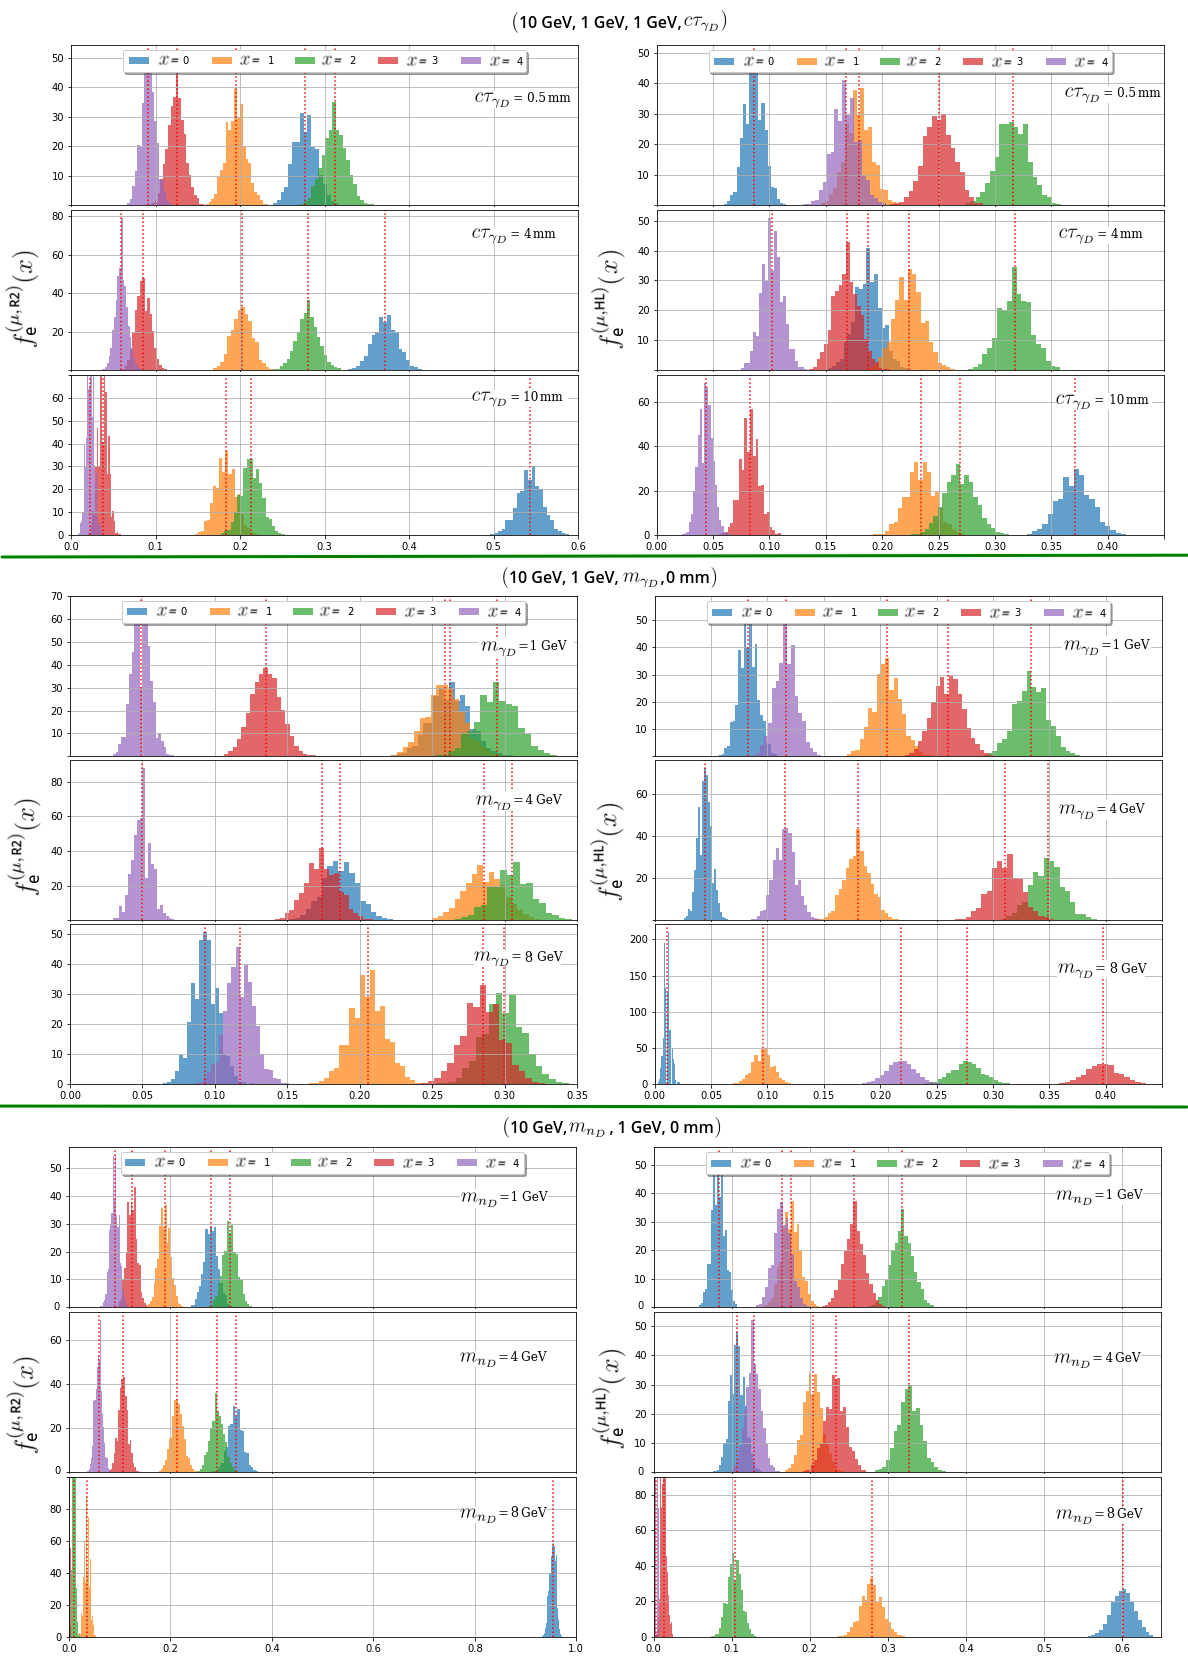
\includegraphics[width=.9\textwidth]{Cap4/imagenes/Distribucion_Entries.png}
\caption{Distribuciones de frecuencias resultado de aplicar ``\textit{bootstrap}'' sobre los valores $f^{(\mu, k)}_\textsf{e} (x)$ ante cambios de los parámetros $\vec{\alpha}$.}
\label{entradas}
\end{figure}

Para entender el sesgo o varianza de un estadístico genérico resultado de su aplicación sobre una población finita $\mathbb{M}$, se aplica el ``\textit{Bootstrapping}''\footnote{Más información en el enlace \href{https://es.wikipedia.org/wiki/Bootstrapping\_(estad\%C3\%ADstica)}{https://\-es.\-wi\-ki\-pe\-dia.\-org/\-wi\-ki/\-Boots\-tra\-pping\_(es\-tad\-\%C3\-\%AD\-sti\-ca)}}. Este método es el resultado de la selección aleatoria de subconjuntos $\mathbb{M}_i\subset \mathbb{M}$, seguida de la aplicación del estadístico sobre esta. La aplicación continua de ``\textit{bootstrap}'' sobre el estadístico $f^{(\mu, k)}_\textsf{e} (x)$ y el graficar los histogramas normalizados resultantes (ver Fig. \ref{entradas}) permitirán entender la correspondencia de los términos $\vec{\alpha}$ con las distribuciones.

En las distribuciones de la Fig. \ref{entradas} se visualiza la alta dependencia con los parámetros de generación $\vec{\alpha}$, además se evidenciaron únicamente $f^{(\mu, k)}_\textsf{e}(5)\lesssim 3\cdot 10^{-5}$ para los cambios considerados en la Tabla  \ref{table_genera_v5_value}, razón por la cual son descartados de este estudio eventos con más de 4 muones. Si consideramos que la forma de estas distribuciones corresponde con una gaussiana, el error en la frecuencia $\Delta f^{(\mu, k)}_\textsf{e} (x) \equiv \Delta f^{(\mu, k)}_\textsf{e} (x;\vec{\alpha})$ de la ec. \ref{fe} es calculable siguiendo la referencia \cite{muestra_1} como:
%f^{(p, k)}_\textsf{e} (\vec{\alpha}; x) = \sum_{i=1}^{N_e} \delta_{x}(n_i^{(p,k)})/\sum_{i=1}^{N_e} \sum_{n=0}^\infty \delta_{n} (n_i^{(p,k)}) = \sum_{i=1}^{N_e} \delta_{x}(n_i^{(p,k)})/N_e
\begin{eqnarray}\label{error0}
\Delta f^{(\mu, k)}_\textsf{e} (x) & = f^{(\mu, k)}_\textsf{e} (x) \cdot Z_{\frac{\beta}{2}} \sqrt{\dfrac{\rho(1-\rho)}{f^{(\mu, k)}_\textsf{e} (x)\cdot N_e}} \\
& = \dfrac{Z_{\frac{\beta}{2}}}{100} \sqrt{\rho(1-\rho)\cdot f^{(\mu, k)}_\textsf{e} (x)} ~~~~~~~~~~~
\end{eqnarray}%\sqrt{\dfrac{\mathbb{E}^{(\mathtt{k})}- \mathbb{E}^{(j,~\mathtt{k})}}{\mathbb{E}^{(\mathtt{k})}-1}}
donde $Z_{\frac{\beta}{2}}$ es un parámetro que depende del nivel de confianza $(1-\beta$), con posibles valores dados por $Z_{\frac{0.1}{2}}=1.65$, $Z_{\frac{0.05}{2}}=1.96$ y $Z_{\frac{0.01}{2}}=2.58$ y $\rho$ es la probabilidad ocurrencia.

Otro elemento importante a tener en cuenta, es la variación de la fracción de muones reconstruidos por los detectores del total \MC, entonces:
\begin{eqnarray}\label{Ak}
A_\textsf{n}^\mu(k) & = {\sum\limits_{i=1}^{N_e} n_i^{(\mu,k)}}/{\sum\limits_{i=1}^{N_e} n_i^{(\mu,\textsf{True})}}
\end{eqnarray}
ejemplos de la variación de este estadístico con el parámetro de generación $\vec{\alpha}$ se encuentran en la Tabla \ref{Numero_de_Entradas}.



\subsubsection{Correspondencia entre los eventos de interés y los parámetros de generación.}
\begin{figure}[!t]
\centering
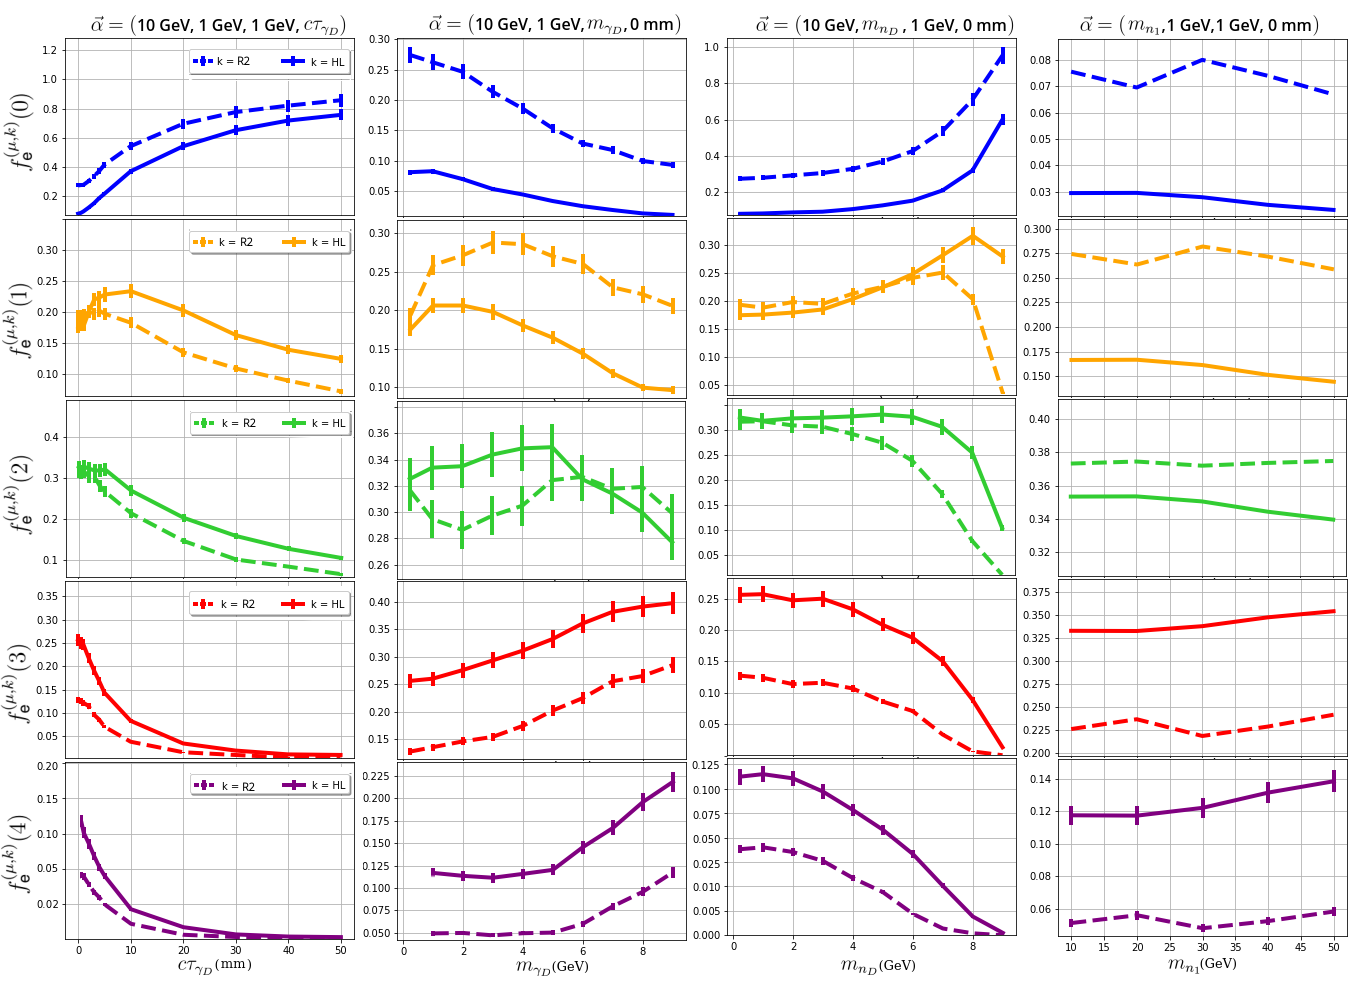
\includegraphics[width=.9\textwidth]{Cap4/imagenes/Comparacion_Distribucion_Entries0.png}
\caption{Ejemplo de variaciones del parámetro $f^{(\mu, k)}_\textsf{e} (\vec{\alpha}; x)$.}
\label{entradasALL}
\end{figure}

Algunos ejemplos de los valores de $f^{(\mu, k)}_\textsf{e} (x)$ los podremos observar en la Tabla \ref{Numero_de_Entradas} y en los gráficos de la Fig. \ref{entradasALL}. En estos se puede observar una clara tendencia con los parámetros de generación $\vec{\alpha}$. Se pudo constatar la disminución de eventos de interés $f^{(\mu, k)}_\textsf{e} (4)$ con el aumento del tiempo de vida del fotón oscuro $c\tau_{\gamma_D}$ y de la masa del neutralino oscuro $m_{n_D}$, en contraste se registra aumento de los eventos de interés con la masa del fotón oscuro $m_{\gamma_D}$. En el caso de cambios de la masa del neutralino ligero $m_{n_1}$, los datos muestran variaciones pequeñas en el rango definido (ver Tabla \ref{table_genera_v5_value}), los datos adquiridos no dan una conclusión clara de su comportamiento.


% Al comparar los resultados podemos observar empíricamente una tendencia de estos valores de frecuencia ante cambios de los parámetros de generación.


%\begin{landscape}
\begin{table}[!t]
\centering
\footnotesize
\begin{tabular}{|cccc|cccc|}
\toprule
\multicolumn{4}{|c|}{$\vec{\alpha}$} & \multicolumn{4}{|c|}{Estadístico} \\
\hline
$m_{n_1}$ & $m_{n_D}$ & $m_{\gamma_D}$ & $c\tau_{\gamma_D}$ & 
$A_n^\mu(\texttt{R2})$ & 
$A_n^\mu(\texttt{HL})$ & 
$f^{(\mu, \texttt{R2})}_\textsf{e} (4)$ & 
$f^{(\mu, \texttt{HL})}_\textsf{e} (4)$ \\
\midrule
10 & 1 & 1 & 0.5 & 0.2908 & 0.4261 & 0.0504 $\pm$ 0.0029& 0.1153 $\pm$ 0.0044\\
& & & 2 & 0.2909 & 0.4250 & 0.0497 $\pm$ 0.0029& 0.1158 $\pm$ 0.0044\\
& & & 4 & 0.2861 & 0.4139 & 0.0468 $\pm$ 0.0028& 0.1152 $\pm$ 0.0044 \\
& & & 10 & 0.2628 & 0.3783 & 0.0380 $\pm$ 0.0025& 0.0939 $\pm$ 0.0039\\
& & & 50 & 0.1330 & 0.2022 & 0.0086 $\pm$ 0.0012& 0.0212 $\pm$ 0.0019\\
& & & 100 & 0.0815 & 0.1311 & 0.0017 $\pm$ 0.0005& 0.0075 $\pm$ 0.0012\\
\midrule
%10 & 0.25 & 0.25 & 0 & 0.2744 $\pm$ 0.0410 & 0.0813 $\pm$ 0.0223 & 0.0881 $\pm$ 0.0232 & 0.1622 $\pm$ 0.0315 \\
10 & 1 & 2 & 0 & 0.3567 & 0.5167 & 0.0509 $\pm$ 0.0029& 0.1102 $\pm$ 0.0043\\
& & 4 & & 0.3893 & 0.5492 & 0.0491 $\pm$ 0.0029& 0.1166 $\pm$ 0.0044\\
& & 6 & & 0.4451 & 0.5991 & 0.0597 $\pm$ 0.0032& 0.1451 $\pm$ 0.0049\\
& & 8 & & 0.4857 & 0.6348 & 0.0854 $\pm$ 0.0038& 0.1882 $\pm$ 0.0056\\
\midrule
10 & 2 & 1 & 0 & 0.3382 & 0.5020 & 0.0464 $\pm$ 0.0028& 0.1110 $\pm$ 0.0043\\
& 4 & & & 0.3072 & 0.4732 & 0.0348 $\pm$ 0.0024& 0.0891 $\pm$ 0.0039\\
& 6 & & & 0.2414 & 0.4142 & 0.0139 $\pm$ 0.0015& 0.0548 $\pm$ 0.0030 \\
& 8 & & & 0.0993 & 0.2732 & 0.0012$\pm$ 0.0004& 0.0108 $\pm$ 0.0013\\
\midrule
20 & 1 & 1 & 0 & -- & -- & 0.0560 $\pm$ 0.0030 & 0.1176 $\pm$ 0.0044 \\
30 & & & &  --  & -- & 0.0480 $\pm$ 0.0028 & 0.1224 $\pm$ 0.0045\\
40 & & & & -- & -- &  0.0524 $\pm$ 0.0030 &  0.1319 $\pm$ 0.0047 \\
50 & & & & -- & -- & 0.0583 $\pm$ 0.0031 & 0.1391 $\pm$ 0.0048 \\
\bottomrule 
\end{tabular}
\caption{Variación de estadísticos característicos para combinaciones de los términos del parámetro generación $\vec{\alpha}$ y los detectores $k$.}
\label{Numero_de_Entradas}
\end{table}



Dado que se intenta reconstruir el decaimiento de la Fig. \ref{fig:sketch_darksector}b, el estadístico $f^{(\mu, k)}_\textsf{e} (x)$ para $x \geq 4$ es el de mayor interés para esta investigación, el mismo muestra como la configuración del detector en Alta Luminosidad ($k=\textsf{HL}$) reconstruye entre 2.2 a 9 veces más de eventos con 4 muones reconstruidos por el detector \CMS ~ en la configuración Run-2 ($k=\textsf{R2}$) para las muestras simuladas (ver Tabla \ref{table_genera_v5_value}).

%%\begin{landscape}
%\begin{table}[!t]
%\centering
%\footnotesize
%\begin{tabular}{|cccc|cccc|}
%\toprule
%\multicolumn{4}{|c|}{$\vec{\alpha}$} & \multicolumn{4}{|c|}{Estadístico} \\
%\hline
%$m_{n_1}$ & $m_{n_D}$ & $m_{\gamma_D}$ & $c\tau_{\gamma_D}$ & 
%$A_n^\mu(\texttt{R2})$ & 
%$A_n^\mu(\texttt{HL})$ & 
%$f^{(\mu, \texttt{R2})}_\textsf{e} (4)$ & 
%$f^{(\mu, \texttt{HL})}_\textsf{e} (4)$ \\
%\midrule
%10 & 1 & 1 & 0.5 & 0.2908 & 0.4261 & 0.0920 $\pm$ 0.0040 & 0.1678 $\pm$ 0.0053\\
%& & & 2 & 0.2909 & 0.4250 & 0.0779 $\pm$ 0.0036 & 0.1355 $\pm$ 0.0047 \\
%& & & 4 & 0.2861 & 0.4139 & 0.0597 $\pm$ 0.0032 & 0.1024 $\pm$ 0.0041\\
%& & & 10 & 0.2628 & 0.3783 & 0.0227 $\pm$ 0.0019 & 0.0433 $\pm$ 0.0027\\
%& & & 50 & 0.1330 & 0.2022 & 0.0016 $\pm$ 0.0005 & 0.0039 $\pm$ 0.0008\\
%& & & 100 & 0.0815 & 0.5111 & 0.0002 $\pm$ 0.0002 & 0.0006 $\pm$ 0.0003\\
%\midrule
%%10 & 0.25 & 0.25 & 0 & 0.2744 $\pm$ 0.0410 & 0.0813 $\pm$ 0.0223 & 0.0881 $\pm$ 0.0232 & 0.1622 $\pm$ 0.0315 \\
%10 & 1 & 2 & 0 & 0.3567 & 0.5167 & 0.0497 $\pm$ 0.0029 & 0.1135 $\pm$ 0.0043 \\
%& & 4 & & 0.3893 & 0.5492 & 0.0494 $\pm$ 0.0029 & 0.1157 $\pm$ 0.0040 \\
%& & 6 & & 0.4451 & 0.5991 & 0.0599 $\pm$ 0.0032 & 0.1456 $\pm$ 0.0049\\
%& & 8 & & 0.4857 & 0.6348 & 0.0957 $\pm$ 0.0040 & 0.1960 $\pm$ 0.0057\\
%\midrule
%10 & 2 & 1 & 0 & 0.3382 & 0.5020 & 0.0852 $\pm$ 0.0038 & 0.1604 $\pm$ 0.0052\\
%& 4 & & & 0.3072 & 0.4732 & 0.0586 $\pm$ 0.0031 & 0.1281 $\pm$ 0.0046 \\
%& 6 & & & 0.2414 & 0.4142 & 0.0221 $\pm$ 0.0019 & 0.0831 $\pm$ 0.0037\\
%& 8 & & & 0.0993 & 0.2732 & 0.0022 $\pm$ 0.0006 & 0.0193 $\pm$ 0.0018\\
%\midrule
%20 & 1 & 1 & 0 & -- & -- & 0.0560 $\pm$ 0.0030 & 0.1176 $\pm$ 0.0044 \\
%30 & & & &  --  & -- & 0.0480 $\pm$ 0.0028 & 0.1224 $\pm$ 0.0045\\
%40 & & & & -- & -- &  0.0524 $\pm$ 0.0030 &  0.1319 $\pm$ 0.0047 \\
%50 & & & & -- & -- & 0.0583 $\pm$ 0.0031 & 0.1391 $\pm$ 0.0048 \\
%\bottomrule 
%\end{tabular}
%\caption{Variación de estadísticos característicos para combinaciones de los términos del parámetro generación $\vec{\alpha}$ y los detectores $k$.}
%\label{Numero_de_Entradas}
%\end{table}



\subsubsection{Regresión de datos de frecuencia}

Con la intención de realizar una caracterización eficiente de la cantidad de eventos de interés y de su dependencia con los parámetros de generación, se intenta utilizar métodos simples de regresión para valorar la posibilidad de inferir información pertinente a la frecuencia de los eventos. Para esto se utilizan los métodos presentados ya en la sección \ref{Cap_regresion} mediante una aproximación lineal como la propuesta en la ec. \ref{regresion} y con una red neuronal como la presentada en la Fig. \ref{neuronas}.

\begin{figure}[!ht]
\centering
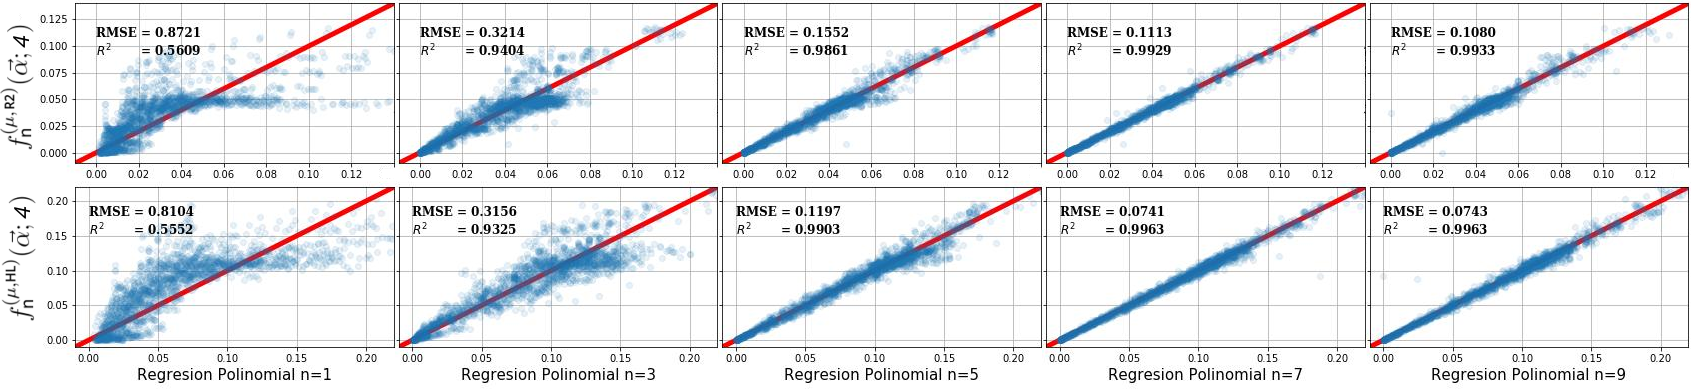
\includegraphics[width=1\textwidth]{Cap4/imagenes/ML_Entries3.png}
\caption{Resultados de la regresión polinomial de los valores de frecuencia $f^{(\mu, k)}_\textsf{e} (4;\vec{\alpha})$.}
\label{regresionALL}
\end{figure}


Al implementar el método de regresión polinomial sobre los datos $f^{(\mu, k)}_\textsf{e} (4)$ hasta el orden $n = 9$ visualizada en la Fig. \ref{regresionALL}, se puede observar una mejora en los parámetros progresiva con el aumento del orden $n$. La correspondencia entre los valores simulados y los predichos es corroborada por los parámetros de confianza \textbf{RMSE} y $\mathbf{R^2}$. 
\begin{figure}[!ht]
\centering
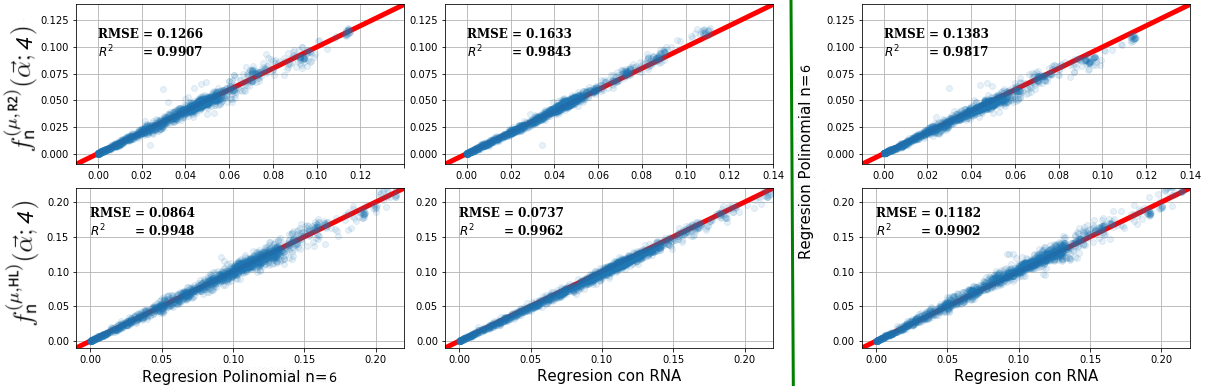
\includegraphics[width=.9\textwidth]{Cap4/imagenes/ML_Entries.png}
\caption{Comparación de los resultados de regresión utilizando RNA y regresión polinomial para predecir las frecuencias $f^{(\mu, k)}_\textsf{e} (4; \vec{\alpha})$.}
\label{regresionALL1}
\end{figure}

Haciendo uso del método \textbf{RNA} según una configuración semejante a la Fig. \ref{regresion} con $6$ capas ocultas con cantidad de nodos dada por $m_k=128,~64,~32,~16,~8,~4$, se obtuvo un modelo con valores de \textbf{RMSE} y $\mathbf{R^2}$ comparables con los del método de regresión lineal explicado con anterioridad.

En la Fig. \ref{regresionALL1} también se puede observar una comparación de los resultados de los dos métodos al intentar reconstruir la información de los valores de frecuencia $f^{(4\mu,~k)}_\textsf{e}$ mostrando una alta linealidad en los resultados obtenidos validando su implementación como método de análisis. Los resultados dan claridad de como el método de predicción de la fracción de eventos con 4 muones del total puede ser utilizado para optimizar la selección del parámetro $N_e$ en el proceso de generación (ver Tabla \ref{table_genera_v5_value}).

%Al analizar los errores de estás predicciones con los datos originales se obtuvo que lo resultados diferencian hasta en un $\sim 30\%$, siendo una de las posibles consecuencias de estos altos errores el pequeño valor del parámetro de generación \texttt{Event} (ver sección \ref{Cap_genera}).

%\begin{landscape}
%\begin{figure}[h]
%\centering
%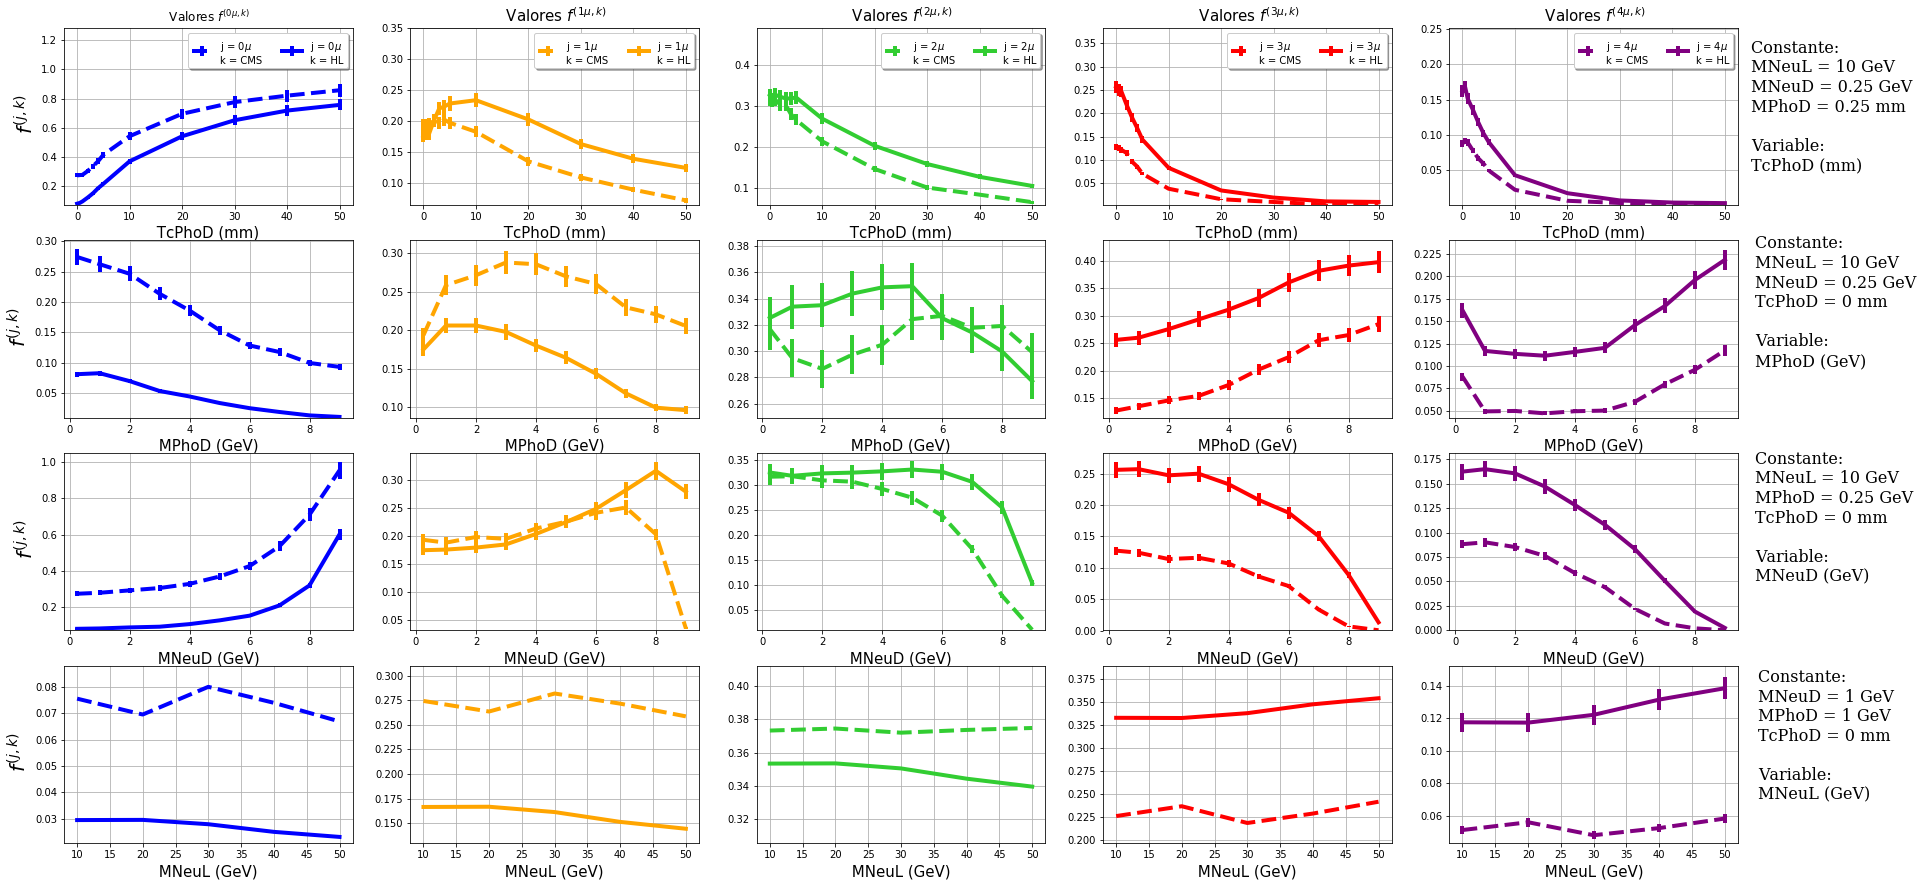
\includegraphics[width=1.2\textwidth]{Simulacion/imagenes/Comparacion_Distribucion_Entries.png}
%\caption{Distribuciones de frecuencia de las entradas $f^{(j,~k)}$ ante cambios de \texttt{MNeuD}.}
%\label{entradasALL}
%
%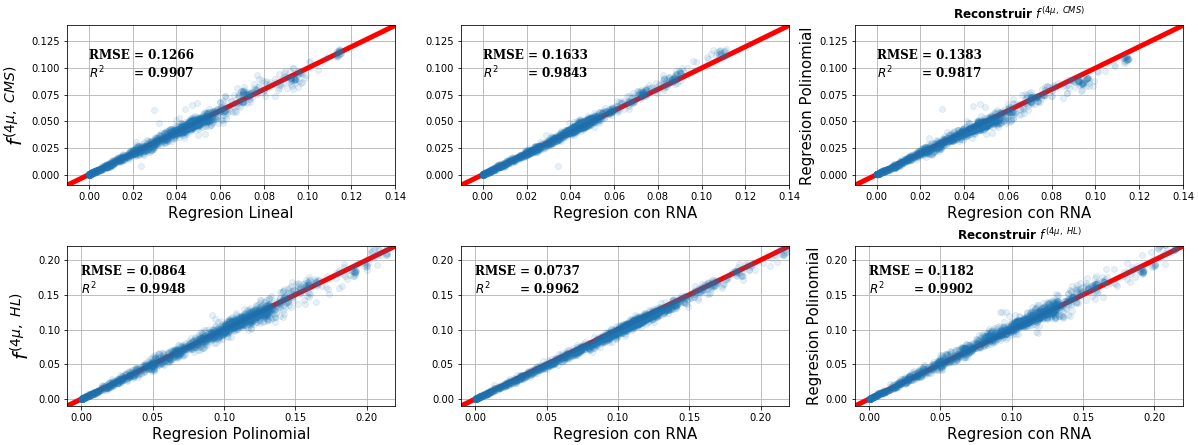
\includegraphics[width=1\textwidth]{Simulacion/imagenes/ML_Entries.png}
%\caption{Resultados de la regresión de los valores de frecuencia $f^{(4\mu,~k)}$.}
%\label{regresionALL}
%\end{figure}
%\end{landscape} 


%\subsubsection{Probabilidad de ocurrencia.}

%Para cierta combinación de parámetros, los detectores en sus diferentes configuraciones tienen una probabilidad $p$ de ocurrencia o reconstrucción del muón, si se hace la suposición de que esta probabilidad es fija para cierta morfologia en las propiedades de los muones entonces podemos hacer uso de la binomial para facilitar las comparaciones entre los eventos.
%Partiendo de la ecuación binomial:
%\begin{equation}\label{binomial}
%f^{(j,~k)} = \dfrac{n_{max}!}{n_j!~(n_{max} - n_j)!} ~ p^{n_j} ~ (1-p)^{n_{max}-n_j}
%\end{equation}
%donde:\\
%\begin{tabular}{lp{14cm}}
%$n_{j} = j$ & número de muones. Para nuestras muestras los valores admisibles son $j = \{0,~1,~2,~3,~4\}$, resultado de lo cual $n_{max} = n_{4\mu} = 4$. \\
%$p$ & es la probabilidad ocurrencia o reconstrucción de los muones.
%\end{tabular}
%Dado que el $\backsim 80\%$ de los datos generados a los que se tiene acceso solo se posee información de los eventos $\mathbb{E}^{(4\mu,~\mathtt{k})}$, entonces podemos calcular la probabilidad de ocurrencia como:
%\begin{equation}\label{ocurrencia}
%f^{(4\mu,~k)} = \dfrac{4!}{4!~0!} ~ p^{4} ~ (1-p)^{0} = p^{4} ~~~\Rightarrow ~~~ p = \sqrt[4]{f^{(4\mu,~k)}}
%\end{equation}
%
%Finalmente sustituyendo la ec. \ref{ocurrencia} en ec. \ref{binomial} tenemos:
%\begin{equation}\label{binomialF}
%f^{(j,~k)} = \dfrac{n_{max}!}{n_j!~(n_{max} - n_j)!} ~ (f^{(4\mu,~k)})^{\frac{n_j}{4}} ~ (1-(f^{(4\mu,~k)})^{\frac{1}{4}})^{n_{max}-n_j}
%\end{equation}
%Con esta ecuación se podrá simular los valores $f^{(j,~k)}$ para los datos con información reducida, aunque dada las suposiciones que deriban de esta ecuación los errores observados de la comparación con los datos reales pueden llegar a $20\%
%,$.%$\Delta f^{(j,~k)} / f^{(j,~k)} = 20\%$ 
%
%
%
%
%

\subsection{Variación de las propiedades de los muones}

\begin{figure}[!t]
\centering
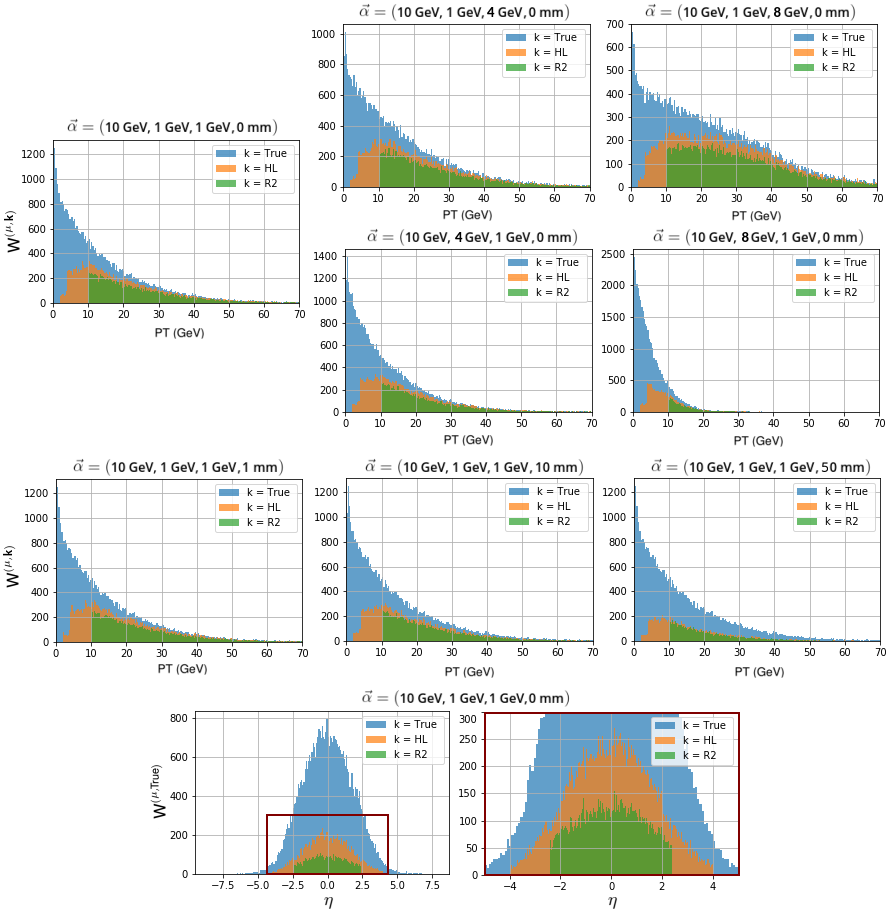
\includegraphics[width=.9\textwidth]{Cap4/imagenes/PT_comparacion.png}
%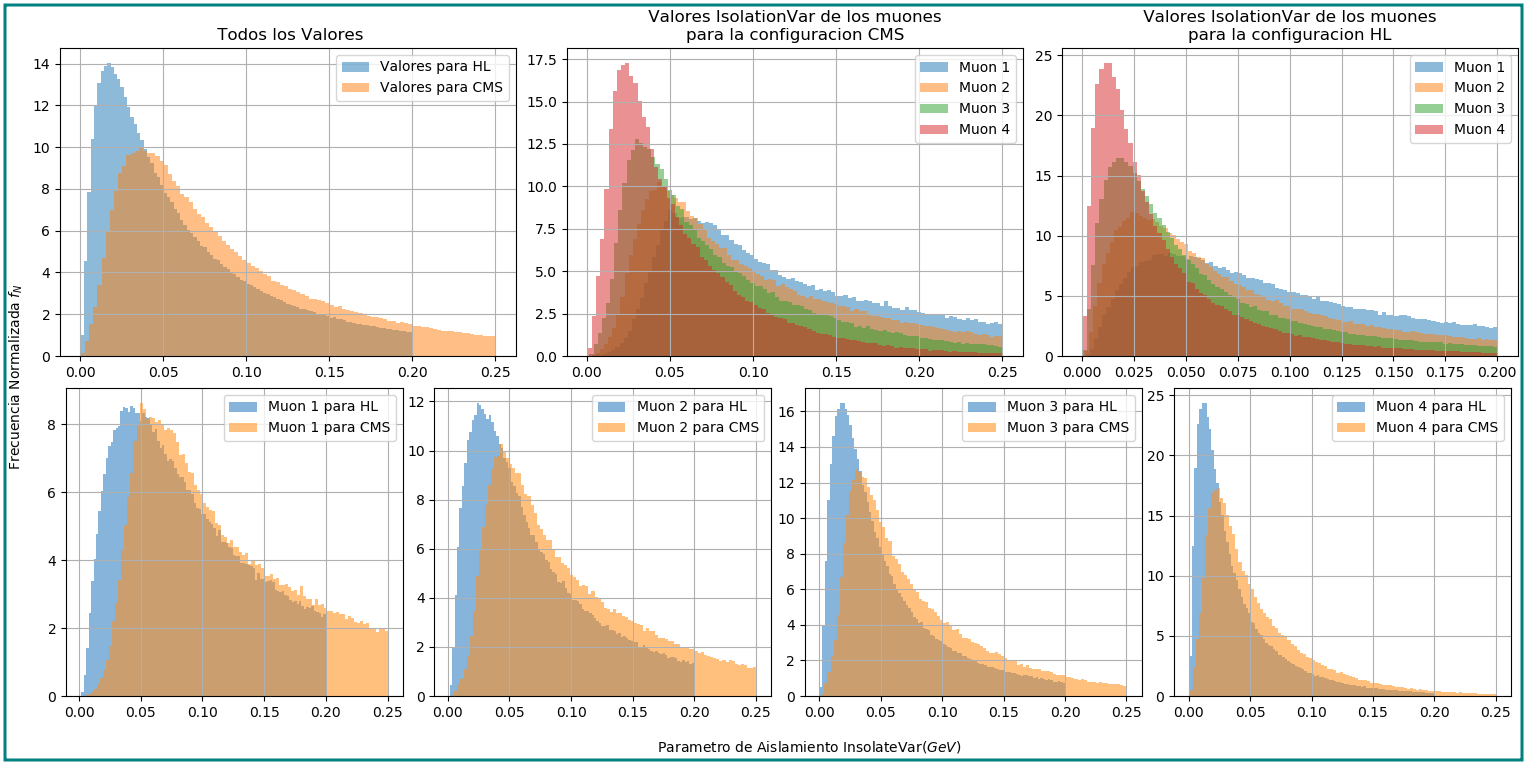
\includegraphics[width=.8\textwidth]{Simulacion/imagenes/Datos_IsolationVar_ALL.png}
\caption{Variación de las propiedades momento transversal y de la pseudorapidez de los muones en diferentes configuraciones del detector $k$ y ante variaciones del parámetro de generación $\vec{\alpha}$.}
\label{Comparacion}
\end{figure}

La caracterización de las propiedades de los muones $ \textsf{W}^{(\mu,k)} ({\textsf{x}_j})$, es parte importante de este estudio, por ello, se analizan las variaciones en la morfología de las distribuciones para las diferentes configuraciones $k=\mathbf{R2}, \mathbf{HL}$ comparadas con la teoría $k=\mathbf{True}$. 

En las distribuciones correspondientes al momento transversal (Fig. \ref{Comparacion}) se encontraron cambios en la morfología con los parámetros $m_{\gamma_D}$ y $m_{n_D}$, mientras que, una variación de la amplitud  en la escala de frecuencias con el parámetro de tiempo de vida del fotón oscuro $c\tau_{\gamma_D}$. Al comparar las distribuciones correspondientes a las diferentes configuraciones de los detectores se comprobó correctamente el aumento en la eficiencia de detección entre $\approx 6\%-14\%$ en la configuración de Alta Luminosidad para valores del momento de $P_T>10 ~GeV$. Además, a diferencia de la configuración Run-2, la configuración en Alta Luminosidad permitirá detectar muones de baja energía, información que será determinante con el aumento teórico del parámetro de masa del neutralino oscuro $m_{n_D}$, estos resultados con congruentes con los presentados en la Tabla \ref{Numero_de_Entradas}.

En la configuración  Run-2 existe un corte para valores de pseudorapidez de $|\eta|\lesssim 2.4$, correspondiéndose al espectro donde se ubican el $\backsim 68\%$ de los muones, por otro lado, en la configuración de Alta Luminosidad se tiene $|\eta|\lesssim 4$, correspondiente al $\backsim 96\%$ de las partículas generadas por la señal \MC. De lo anterior queda claro que la mejora esperada en el experimento \CMS, será determinante en la localización de las partículas provenientes de la teoría \MSSM\textbf{D}.

\subsection{Reconstruyendo el fotón oscuro}
Se está investigando el decaimiento $h \rightarrow 2n_1 \rightarrow 2n_D + 2\gamma_D \rightarrow 2n_D + 4\mu$ correspondiente al proceso \textbf{Dark-}\SUSY ~ o \MSSM\textbf{D} como se muestra en el diagrama de la Fig. \ref{fig:sketch_darksector}b. Se aplicaron 3 métodos diferentes para calcular la masa del fotón oscuro $\gamma_D$ correspondiente a este decaimiento. Estos métodos son comparados y caracterizados, se analizan sus ventajas y limitaciones.

%, para poder reconstruir el fotón oscuro $\gamma_D$ se hará uso de los eventos característicos del estadístico $f^{(\mu, k)}_\textsf{e} (4;\vec{\alpha})$ ya que estos poseen la información necesaria para ello. Una de las problemáticas importantes a tener en cuenta en esta investigación es la reconstrucción del fotón oscuro con la mayor fiabilidad posible, para ello métodos que permitán disminuir los errores se hacen necesario. 


\subsubsection{Método $\mathbb{N}_\textsf{True}$}
%$\mathbb{N}_\textsf{True}$ 
%En los archivos $\textsf{*.root}$ 
Hace referencia a la comparación directa por eventos de la información contenida en la rama $\textsf{\small Particle}$ y la rama $\textsf{\small Muon}$ del archivo $\textsf{\small *.root}$. La primera, se obtiene de la clase $\textsf{\small GenParticle}$ la cual contiene la información de las partículas generadas con \MC ~ ($k=\textsf{\small True}$); mientras que la segunda, obtenida por la clase $\textsf{\small Muon}$, proporciona las propiedades de los muones detectados mediante el proceso de simulación del detector en la configuración elegida. $k=\textsf{\small HL, R2}$. %Para reconocer el origen en la simulación de los muones reconstruidos por el detector, se hace necesario una comparación entre los muones generados y los detectados, sabido que estos poseen variaciones en sus propiedades resultado de los errores instrumentales. 
Para detectar el origen de las partículas que son reconstruidas por el detector se implementa un proceso iterativo de comparación entre los muones del detector y los generados. Se considera que es el mismo muon simulado por \MC~$\mu_1$ y el reconstruido por el detector $\mu_2$ aquel que cumple con lo siguiente: 
\begin{itemize_f}
\item La diferencia en el momento transversal sea menor al 10\% de la media:
\begin{equation}\label{q1}
2\cdot \dfrac{\left|P_T^{(\mu_1)}-P_T^{(\mu_2)}\right|}{P_T^{(\mu_1)}+P_T^{(\mu_2)}} < 0.1
\end{equation} 
\item La distancia entre las partículas en el plano $\eta \times \phi$ sea mínima:
\begin{equation}\label{q2}
\min{(\Delta R)} = \sqrt{\left(\eta^{(\mu_1)} - \eta^{(\mu_2)}\right)^2 + \left(\phi^{(\mu_1)} - \phi^{(\mu_2)}\right)^2}
\end{equation}
\end{itemize_f} 
%Dado que el origen de las partículas dentro de la rama $\textsf{\small Particles}$ ($k=\textsf{\small True}$) del archivo $\textsf{*.root}$ es determinado dentro de las variables $\textsf{Particles.M1}$, 
Estos criterios dados por las ecs. \ref{q1} y \ref{q2} permiten conocer el origen de los muones reconstruidos por el detector (dentro de la rama $\textsf{\small Muon}$), con bajo porcentaje de error. Este método permite conocer el origen individual de cada muon con alta fiabilidad. Entre sus desventajas se encuentra la imposibilidad de conocer los errores resultados de la comparación. %Su aplicación solo es posible ante datos simulados.

\subsubsection{Aplicando el método $\mathbb{N}_\textsf{True}$}


\begin{figure}[!t]
\centering
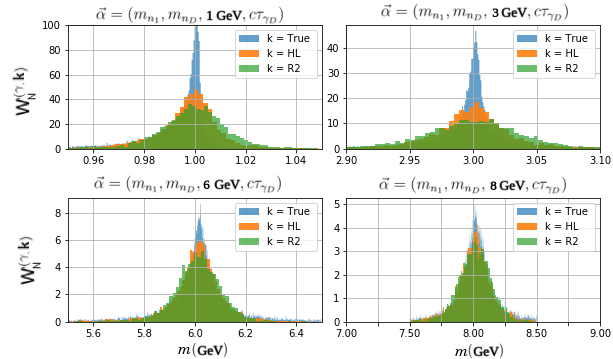
\includegraphics[width=.95\textwidth]{Cap4/imagenes/foton_mass.png}
%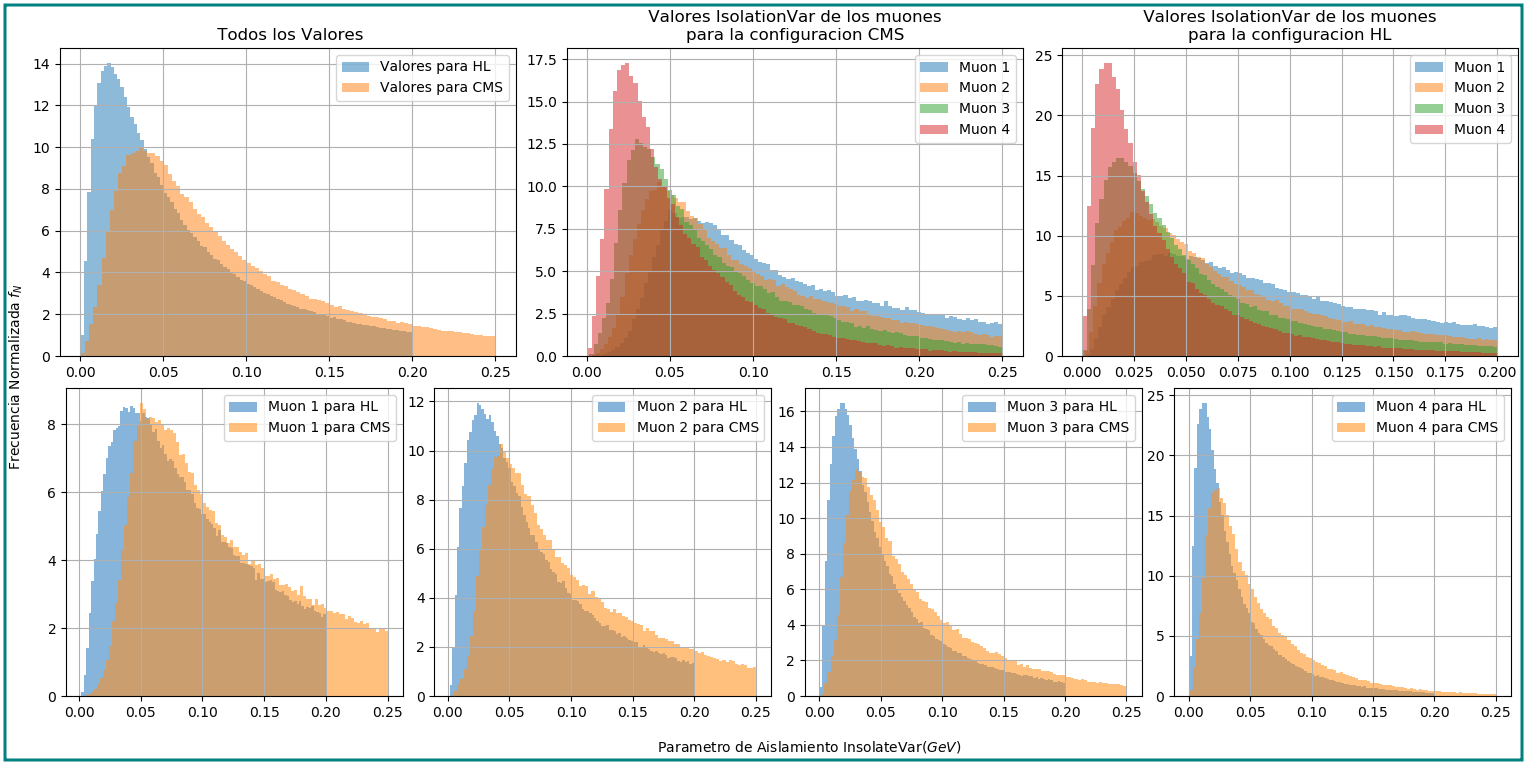
\includegraphics[width=.8\textwidth]{Simulacion/imagenes/Datos_IsolationVar_ALL.png}
\caption{Valores de masa invariante reconstruida de di-muones identificados con el método $\mathbb{N}_\textsf{True}$.}
\label{mass_inv}
%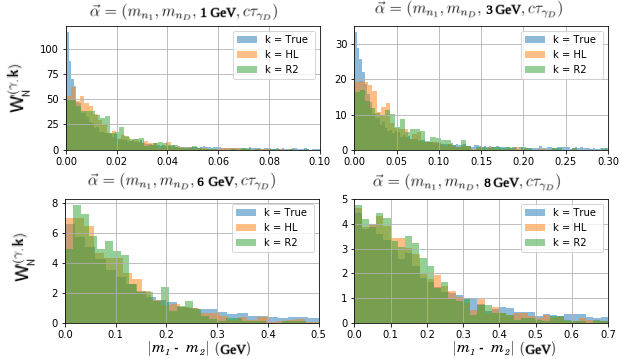
\includegraphics[width=.95\textwidth]{Simulacion/imagenes/foton_mass_diff.png}
%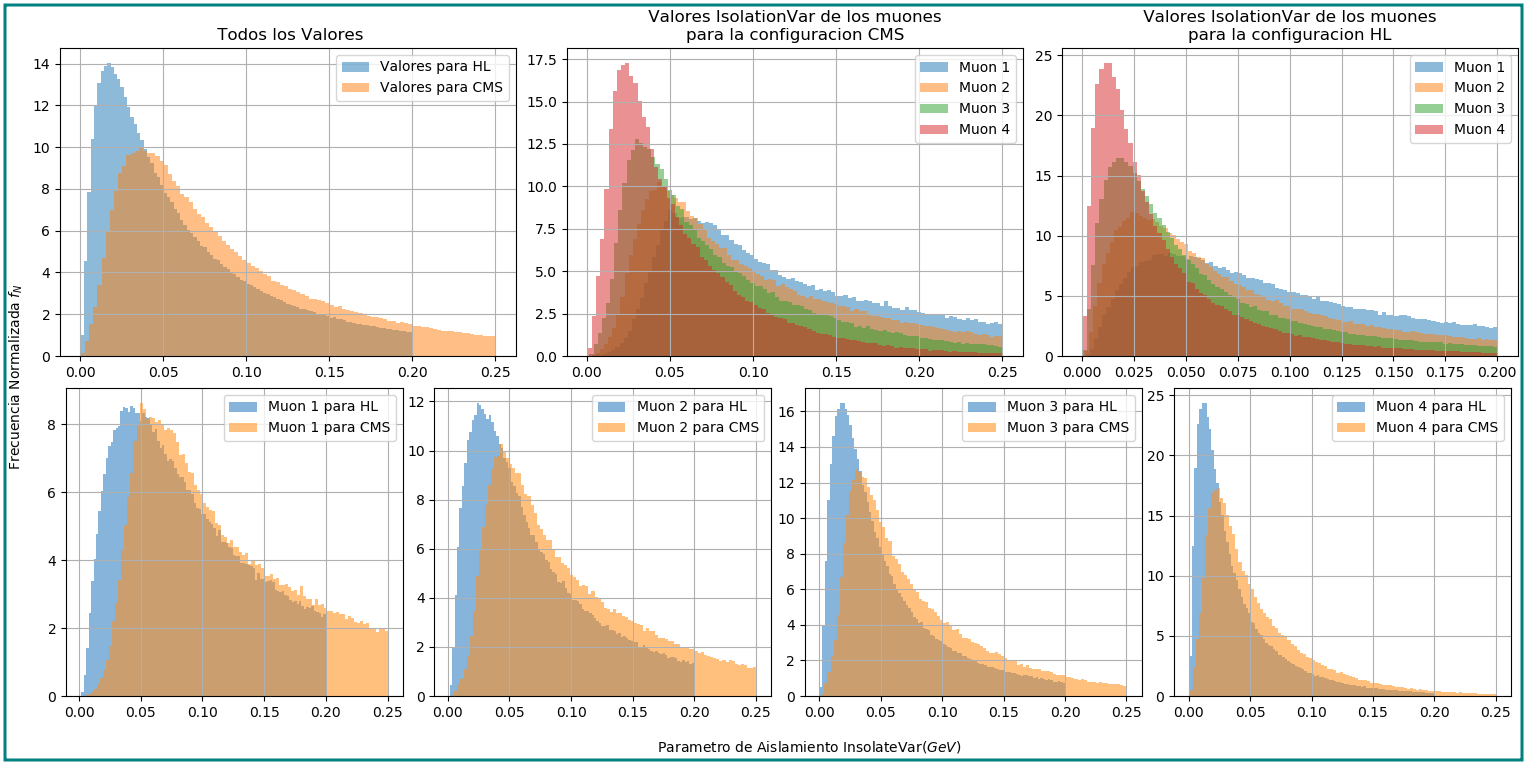
\includegraphics[width=.8\textwidth]{Simulacion/imagenes/Datos_IsolationVar_ALL.png}
%\caption{.}
%\label{mass_inv2}
\end{figure}

%\begin{landscape}
\begin{table}[!t]
\centering
\footnotesize%small%scriptsize
\begin{tabular}{|c|cc|cc|cc|}
\toprule
Parámetro& \multicolumn{6}{c|}{Rango para el 95\% de los valores de $W_N^{(\gamma_D, ~ k)}$ }\\
$m_{\gamma_D}$ & \multicolumn{2}{c}{$\mathbf{k = True}$} & \multicolumn{2}{c}{$\mathbf{k = HL}$} & \multicolumn{2}{c|}{$\mathbf{k = R2}$}\\
(GeV)
& $\widetilde{m}^{~p_{97.5}(m)}_{~p_{2.5}{(m)}}$ & $p_{95}{(\Delta m)}$
& $\widetilde{m}^{~p_{97.5}{(m)}}_{~p_{2.5}{(m)}}$ & $p_{95}{(\Delta m)}$ 
& $\widetilde{m}^{~p_{97.5}{(m)}}_{~p_{2.5}{(m)}}$ & $p_{95}{(\Delta m)}$ \\
\midrule
1 & $1.0070^{~1.1640}_{~0.9348}$ & 0.0649 & $0.9788^{~1.9138}_{~0.6466}$ & 1.2084 & $0.9972^{~2.3029}_{~0.6101}$ & 1.5625 \\ \midrule
2 & $1.9982^{~2.1223}_{~1.9065}$ & 0.1691 & $1.9884^{~2.7434}_{~1.5316}$ & 1.3099 & $1.9922^{3.0688}_{1.4182}$ & 1.6612\\ \midrule
3 & $2.9952^{~3.2272}_{~2.8510}$ & 0.3650 & $2.9905^{~3.6505}_{~2.5030}$ & 1.2725 & $2.9931^{~3.9416}_{~2.3468}$ & 1.6937\\ \midrule
4 & $4.0082^{~4.3908}_{~3.7929}$ & 0.5377 & $3.9909^{~4.5739}_{~3.4980}$ & 1.2403 & $3.9922^{~4.8446}_{~3.3280}$ & 1.6519\\ \midrule
5 & $5.0256^{~5.4876}_{~4.7461}$ & 0.6704 & $4.9916^{~5.5281}_{~4.5122}$ & 1.2048 & $4.9918^{~5.7624}_{~4.3372}$ & 1.5825 \\ \midrule
6 & $6.0373^{~6.5383}_{~5.6921}$ & 0.8072 & $5.9906^{~6.5903}_{~5.4170}$ & 1.3376 & $5.9897^{~6.8303}_{~5.2344}$ & 1.7378\\ \midrule
7 & $7.0193^{~7.6389}_{~6.6202}$ & 0.9784 & $6.9896^{~7.5784}_{~6.3953}$ & 1.3150 & $6.9897^{~7.7884}_{~6.2239}$ & 1.6676\\ \midrule
8 & $8.0253^{~8.7370}_{~7.5903}$ & 1.0795 & $7.9887^{~8.5680}_{~7.3765}$ & 1.3426 & $7.9858^{~8.7652}_{~7.2176}$ & 1.6717\\
\bottomrule 
\end{tabular}
\caption{Estadísticos característicos para combinaciones de los términos del parámetro generación $\vec{\alpha}$ y los detectores $k$. Los valores de masa se dan en GeV.}
\label{mass0}
\end{table}

Se hace una caracterización general que reúne en grupos todas las muestras simuladas para diferentes valores arbitrarios del parámetro de masa del fotón oscuro específico $m_{\gamma_D}$. A estos grupos se les aplica el proceso de comparación siguiendo el método $\mathbb{N}_\textsf{True}$, y una vez identificados los di-muones reconstruidos se calcula masa invariante $m$. Algunos ejemplos son graficados en la Fig. \ref{mass_inv} y los valores de percentiles $p_{2.5}(m)$ y $p_{97.5}(m)$ de las distribuciones de masa invariante se muestran en la Tabla \ref{mass0}. Además, para diferentes $k$ se calcula el valor correspondiente a la diferencia de las masas invariantes de los di-muones $\Delta m\equiv|m_1-m_2|$ siempre que sea posible reconstruir completamente el decaimiento en el evento, y con el percentil $p_{95}(\Delta m )$ dando una cota superior, reportado en la Tabla \ref{mass0}.

Las distribuciones $W_N^{(\gamma_D,k)}$ para la masa invariante $m$ de los di-muones son en general asimétricas. Además, basado en los resultados de la Tabla \ref{mass0} se pudo comprobar una disminución de los errores y por lo tanto una mejor reconstrucción de la teoría, con el aumento de la masa teórica del fotón oscuro $\gamma_D$. También, la actualización del detector en la configuración $\mathbf{k = HL}$ muestra una disminución entre un $\backsim 21\%-28\%$ en los errores de los valores de masa para el 95\% de los datos. 



\subsubsection{Método $\mathbb{N}_\textsf{RNA}$}
Una vez entrenado el identificador de di-muones (sección \ref{identificador_sec}) %con la información contenida en la rama $\textsf{\small Particle}$ del archivo $\textsf{\small *.root}$
, se aplica un proceso iterativo a todo emparejamiento posible entre los muones reconstruidos por el detector. El emparejamiento se realiza sobre los mejores candidatos determinados bajo una mayor probabilidad% siempre cumpliendo el requisito  mínimo de 0.5 
. La precisión $\textsf{acc}_\textsf{RNA}$ dada por la ecuación \ref{acc}, es obtenida al comparar los emparejamientos realizados con los obtenidos con el método $\mathbb{N}_\textsf{True}$.

Este es un método general que permite su aplicación sobre todos los eventos siempre que se tenga al menos dos muones de cargas opuestas. %Su fiabilidad es calculable al comparar los resultados obtenidos con el método $\mathbb{N}_\textsf{True}$. 
Entre sus desventajas se encuentra que solo puede discernir sobre la pertenencia de los di-muones de un decaimiento \textbf{Dark-}\SUSY, es decir, la caracterización individual de los muones no es posible.

\subsubsection{Método $\mathbb{N}_\textsf{ite}$}
 
Se aplica un proceso iterativo sobre los eventos con un mínimo de 2 muones con carga positiva y 2 de carga negativa. Se emparejan todos los di-muones sin elemento en común de tal forma que la diferencia entre las masas invariantes $m$ resultantes sea mínima:
\begin{equation}
\Delta m_{\min} \equiv \min{(\Delta m)}  = \min{(|m_1-m_2|)}
\end{equation}
A este método se le puede anexar un corte que haga coherente la hipótesis de que los di-muones provienen de la misma partícula teórica, su aplicación implica que $\mathbb{N}_\textsf{ite} \rightarrow \mathbb{N}_\textsf{ite}(\delta m)$, donde $\delta m > \Delta m_{\min}$ hace referencia al valor máximo admisible para la diferencia de masas invariantes. Como resultado del método $\mathbb{N}_\textsf{True}$ (ver Tabla \ref{mass0}) se hace supuesto que un mínimo de 95\% de los pares de di-muones cumplen con $\delta m \approx 2$ GeV para todas las muestras utilizadas en esta investigación. La precisión del método esta dada por $\textsf{acc}_\textsf{ite}$ definida por la ecuación \ref{acc}, es obtenida al comparar los emparejamientos realizados con los obtenidos con el método $\mathbb{N}_\textsf{True}$.
%La frecuencia del error al emparejar incorrectamente los elementos del di-muon es denotada como $\varepsilon_\textsf{ite}$.
Este es un método general, fácilmente reproducible. %Su fiabilidad es calculable al comparar los resultados obtenidos con el método $\mathbb{N}_\textsf{True}$. 
Una desventaja es que solo puede implementarse  a la fracción de muones dada por $f^{(\mu, \texttt{k})}_\textsf{e} (4)$.


\subsubsection{Comparando los métodos $\mathbb{N}_\textsf{True}$, $\mathbb{N}_\textsf{RNA}$ y $\mathbb{N}_\textsf{ite}$}
Se implementa los métodos de análisis especificados en las secciones anteriores sobre el conjunto de datos simulados (ver Tabla \ref{table_genera_v5_value}). Estos, en general, están dirigidos a reconstruir la mayor cantidad de fotones oscuros posibles. La fracción del total generado de fotones oscuros reconstruidos está dada por:
\begin{equation}
A_\textsf{n}^{\gamma_D} (k) = \dfrac{\sum\limits_{i=1}^{N_e} n_i^{(\gamma_D,k)}}{\sum\limits_{i=1}^{N_e} n_i^{(\gamma_D,\textsf{True})}} = \dfrac{1}{2 N_e} \sum\limits_{i=1}^{N_e} n_i^{(\gamma_D,k)}
\end{equation}
donde $i$ hace referencia al evento, $\textsf{n} =\textsf{\small True, RNA, ite}$ es el método, y $k$ a la configuración del detector implementado. 

La cantidad de fotones reconstruidos dependerá del método utilizado para identificarlos y reconstruirlos. Además, con alta fiabilidad se puede considerar que los obtenidos como resultados de implementar $\mathbb{N}_\textsf{True}$ será el tope máximo de fotones oscuros que podrán reconstruirse correctamente. Algunos ejemplos se muestran en la Tabla \ref{fotones_reconstruidos}.
La razón $A_\textsf{True}^{\gamma_D} (\textsf{HL})/A_\textsf{True}^{\gamma_D} (\textsf{R2})$ %para $\mathbb{N}_\textsf{True}$ 
aumenta con los parámetros de generación $c\tau_{\gamma_D}$ y $m_{n_D}$ hasta $\sim 2.2$ y $\sim 4.2$ para 100 mm y 8 GeV respectivamente. La superposición de ambas condiciones resultará en un aumento aún mayor de la razón reportada de forma individual, dado que las causas que las originan son independientes entre sí. De aquí que se ve la importancia en la actualización del experimento \CMS~ ante la posibilidad de que estas condiciones sean las correctas experimentalmente. La correcta identificación de los di-muones emparejados por los diferentes métodos está dada por:
\begin{equation}\label{en}
\epsilon_\textsf{n} = \dfrac{A_\textsf{n}^{\gamma_D} (\textsf{k})\cdot \textsf{acc}_\textsf{n}}{A_\textsf{True}^{\gamma_D} (\textsf{k}) } 
\end{equation}
El método $\mathbb{N}_\textsf{RNA}$ logra identificar correctamente entre el $92\% \lesssim \epsilon_{\textsf{RNA}} \lesssim 99\%$ del total de fotones oscuros que son posibles reconstruir. Por su parte, el método $\mathbb{N}_\textsf{ite}$ %es mayormente más exacto (valor de $\epsilon_{\textsf{ite}}>\textsf{acc}_{\textsf{RNA}}$) en la identificación, 
del total de reconstrucción posible por la teoría, logra detectar entre 
$3.5 \% \lesssim \epsilon_{\textsf{ite}}\lesssim 30\%$ en la configuración Run-2 y $8 \% \lesssim \epsilon_{\textsf{ite}}\lesssim 44\%$ en la configuración Alta Luminosidad, siendo esta dependiente de las condiciones iniciales de generación $\vec{\alpha}$ que rigen la probabilidad de reconstruir correctamente eventos $f^{(\mu, \texttt{k})}_\textsf{e} (4)$ (ver Tabla \ref{Numero_de_Entradas}). Los errores esperados son semejantes a los obtenidos en la Tabla \ref{mass0}, además, no varían de forma importante con los cambios de los parámetros de generación $m_{n_D}$, $m_{n_1}$ y $c\tau_{\gamma_D}$.


\begin{landscape}
\begin{table}[!t]
\centering
\footnotesize
\begin{tabular}{|cccc|c|cc|cc|c|cc|cc|}
\toprule
\multicolumn{4}{|c|}{Parámetro de generación $\vec{\alpha}$} & 
\multicolumn{5}{c}{Configuración Run-2%$\textsf{R2}$
} & \multicolumn{5}{c|}{Configuración Alta Luminosidad%$\textsf{HL}$
}\\
\hline
$m_{n_1}$ & $m_{n_D}$ & $m_{\gamma_D}$ & $c\tau_{\gamma_D}$ &
$\mathbb{N}_\textsf{True}$ &
\multicolumn{2}{c}{$\mathbb{N}_\textsf{RNA}$} & 
\multicolumn{2}{|c|}{$\mathbb{N}_\textsf{ite}$} & 
$\mathbb{N}_\textsf{True}$ &
\multicolumn{2}{c}{$\mathbb{N}_\textsf{RNA}$} & 
\multicolumn{2}{|c|}{$\mathbb{N}_\textsf{ite}$}\\
(GeV) & (GeV) & (GeV) & (mm) & 
$A_\textsf{True}^{\gamma_D} (\textsf{R2})$ & $A_\textsf{RNA}^{\gamma_D} (\textsf{R2})$ & $\textsf{acc}_\textsf{RNA}$ & $A_\textsf{ite}^{\gamma_D} (\textsf{R2})$ & $\textsf{acc}_\textsf{ite}$ & 
$A_\textsf{True}^{\gamma_D} (\textsf{HL})$ & $A_\textsf{RNA}^{\gamma_D} (\textsf{HL})$ & $\textsf{acc}_\textsf{RNA}$ & $A_\textsf{ite}^{\gamma_D} (\textsf{HL})$ & $\textsf{acc}_\textsf{ite}$\\
\midrule
10 	& 1 & 1 & 0 	& 0.2179& 0.2171& 0.9901& 0.0512& 0.9980& 0.3376& 0.3364& 0.9894& 0.1174& 0.9983\\
  	&   &   & 0.5 	& 0.2178& 0.2068& 0.9859& 0.0504& 0.9940& 0.3401& 0.3388& 0.9876& 0.1152& 0.9974\\
	& 	& 	& 1		& 0.2138& 0.2136& 0.9867& 0.0478& 0.9937& 0.3362& 0.3346& 0.9891& 0.1168& 0.9983\\
	& 	& 	& 2		& 0.2171& 0.2169& 0.9871& 0.0498& 0.9939& 0.3390& 0.3382& 0.9867& 0.1158& 0.9965\\
	&	&	& 3 	& 0.2147& 0.2143& 0.9865& 0.0492& 0.9918& 0.3276& 0.3270& 0.9877& 0.1100& 0.9890\\
	& 	& 	& 4		& 0.2107& 0.2100& 0.9857& 0.0468& 0.9936& 0.3269& 0.3256& 0.9872& 0.1152& 0.9852\\
	& 	& 	& 5		& 0.2119& 0.2116& 0.9861& 0.0478& 0.9811& 0.3256& 0.3242& 0.9895& 0.1078& 0.9786\\
	&	&	& 10	& 0.1891& 0.1883& 0.9886& 0.0380& 0.9736& 0.2923& 0.2904& 0.9912& 0.0936& 0.9765\\
	&	&	& 50 	& 0.0838& 0.0836& 0.9910& 0.0086& 0.9418& 0.1424& 0.1422& 0.9894& 0.0212& 0.9811\\
	&	&	& 100 	& 0.0502& 0.0497& 0.9990& 0.0018& 0.8824& 0.0912& 0.0901& 0.9894& 0.0074& 0.9766\\
\midrule
10 	& 1 & 2 & 0 	& 0.2138& 0.2129& 0.9904& 0.0508& 0.9961& 0.3292& 0.3254& 0.9932& 0.1100& 0.9973\\
	& 	& 3 & 		& 0.2130& 0.2113& 0.9886& 0.0478& 0.9937& 0.3342& 0.3290& 0.9898& 0.1139& 0.9974\\
	& 	& 4 & 		& 0.2096& 0.2070& 0.9869& 0.0490& 1.0000& 0.3345& 0.3279& 0.9888& 0.1164& 0.9982\\
	& 	& 5 & 		& 0.2208& 0.2175& 0.9843& 0.0512& 0.9961& 0.3520& 0.3424& 0.9896& 0.1238& 0.9943\\
	&	& 6 &		& 0.2372& 0.2316& 0.9859& 0.0598& 0.9899& 0.3795& 0.3667& 0.9908& 0.1450& 0.9973\\
	& 	& 7 & 		& 0.2641& 0.2569& 0.9889& 0.0732& 0.9983& 0.4072& 0.3924& 0.9912& 0.1641& 0.9951\\
	&	& 8 & 		& 0.2866& 0.2796& 0.9851& 0.0854& 0.9953& 0.4260& 0.4107& 0.9906& 0.1879& 0.9957\\
\midrule
10 	& 2 & 1 & 0 	& 0.2085& 0.2085& 0.9889& 0.0464& 0.9957& 0.3310& 0.3303& 0.9912& 0.1108& 0.9990\\
	& 3 & 	& 		& 0.1972& 0.1971& 0.9895& 0.0440& 1.0000& 0.3166& 0.3159& 0.9913& 0.1020& 0.9990\\
	& 4 & 	& 		& 0.1757& 0.1757& 0.9880& 0.0348& 0.9971& 0.2959& 0.2954& 0.9903& 0.0889& 0.9988\\
	& 5 & 	& 		& 0.1474& 0.1475& 0.9891& 0.0232& 0.9957& 0.2702& 0.2694& 0.9909& 0.0734& 1.0000\\
	& 6 & 	& 		& 0.1165& 0.1170& 0.9850& 0.0140& 1.0000& 0.2310& 0.2304& 0.9883& 0.0547& 0.9982\\
	& 7 & 	& 		& 0.0652& 0.0656& 0.9756& 0.0048& 1.0000& 0.1776& 0.1773& 0.9853& 0.0347& 1.0000\\
	& 8 & 	& 		& 0.0238& 0.0247& 0.9272& 0.0012& 1.0000& 0.1010& 0.1013& 0.9758& 0.0108& 1.0000\\
\midrule
20 	& 1 & 1 & 0 	& 0.0550& 0.0545& 0.9509& 0.0540& 0.9880& 0.1136& 0.1126& 0.9804& 0.1101& 0.9931\\
30 	& 	& 	& 		& 0.0443& 0.0440& 0.9903& 0.0439& 0.9901& 0.1220& 0.1220&	0.9790& 0.1102& 0.9895\\
40 	& 	& 	& 		& 0.0509& 0.0506& 0.9781& 0.0499& 0.9712& 0.1311& 0.1305& 0.9527&	0.1300& 0.9970\\
50 	& 	& 	& 		& 0.0541& 0.0506& 0.9870& 0.0521& 0.9877& 0.1309& 0.1295&	0.9790&	0.1259& 0.9742\\
\bottomrule 
\end{tabular}
\caption{Aplicación de los métodos de reconstrucción del fotón oscuro $\gamma_D$.}
\label{fotones_reconstruidos}
\end{table}
\end{landscape} 













%En los archivos $\textsf{*.root}$ la clase $\textsf{GenParticle}$ posee toda la información relativa a las partículas generadas $k=\textsf{True}$ de nuestra señal \textbf{Dark-}\SUSY ~ y con la clase $\textsf{Muon}$ se accede a la información resultado del proceso de hadronización y simulación del detector en la configuración que fue elegida en el proceso de generación de los eventos $k=\textsf{HL,R2}$. Para reconocer el origen en la simulación de los muones reconstruidos por el detector, se hace necesario una comparación entre los muones generados y los detectados, sabido que estos poseen variaciones en sus propiedades resultado de los errores instrumentales. Para detectar su origen con cierta fiabilidad una proceso iterativo de comparación entre los muones del detector y los generados se hace necesario, este emparejamiento se realiza por evento, y cumple con los requisitos:
%\begin{enumerate}
%\item Encontrar muones en los que sus momentos transversales deben cumplir:
%\begin{equation}
%10~\textsf{GeV}~<|P_T^{(\mu,\textsf{True})}-P_T^{(\mu,\textsf{HL}/\textsf{R2})}|
%\end{equation}
%\item Emparejar muones en el que cumplan con la minimización del valor $\min(\Delta R)$, donde:
%\begin{equation}
%\Delta R = \sqrt{(\eta^{(\mu,\textsf{True})} - \eta^{(\mu,\textsf{HL}/\textsf{R2})})^2 + })
%\end{equation}
%\end{enumerate}




%%\begin{landscape}
%\begin{table}[!t]
%\centering
%\scriptsize
%\begin{tabular}{|c|cccccc|}
%\toprule
%Parámetro& \multicolumn{6}{c|}{Rango para el 95\% de los valores de $W_N^{(\gamma, ~ k)}$ }\\
%$m_{\gamma_D}$ & \multicolumn{2}{c}{$\mathbf{k = True}$} & \multicolumn{2}{c}{$\mathbf{k = HL}$} & \multicolumn{2}{c|}{$\mathbf{k = R2}$}\\
%& $\widetilde{m} \pm \Delta m$ & $\max{|m_1 - m_2|}$ & $\widetilde{m} \pm \Delta m$ & $\max{|m_1 - m_2|}$ & $\widetilde{m} \pm \Delta m$ & $\max{|m_1 - m_2|}$\\
%\midrule
%1 & $1.0070^{1.1640}_{0.9348}$ & 0.0649 & $0.9788^{1.9138}_{0.6466}$ & 1.2084 & $0.9972^{2.3029}_{0.6101}$ & 1.5625 \\ \midrule
%2 & $1.9982^{2.1223}_{1.9065}$ & 0.1691 & $1.9884^{2.7434}_{1.5316}$ & 1.3099 & $1.9922^{3.0688}_{1.4182}$ & 1.6612\\ \midrule
%3 & $2.9952^{3.2272}_{2.8510}$ & 0.3650 & $2.9905^{3.6505}_{2.5030}$ & 1.2725 & $2.9931^{3.9416}_{2.3468}$ & 1.6937\\ \midrule
%4 & $4.0082^{4.3908}_{3.7929}$ & 0.5377 & $3.9909^{4.5739}_{3.4980}$ & 1.2403 & $3.9922^{4.8446}_{3.3280}$ & 1.6519\\ \midrule
%5 & $5.0256^{5.4876}_{4.7461}$ & 0.6704 & $4.9916^{5.5281}_{4.5122}$ & 1.2048 & $4.9918^{5.7624}_{4.3372}$ & 1.5825 \\ \midrule
%6 & $6.0373^{6.5383}_{5.6921}$ & 0.8072 & $5.9906^{6.5903}_{5.4170}$ & 1.3376 & $5.9897^{6.8303}_{5.2344}$ & 1.7378\\ \midrule
%7 & $7.0193^{7.6389}_{6.6202}$ & 0.9784 & $6.9896^{7.5784}_{6.3953}$ & 1.3150 & $6.9897^{7.7884}_{6.2239}$ & 1.6676\\ \midrule
%8 & $8.0253^{8.7370}_{7.5903}$ & 1.0795 & $7.9887^{8.5680}_{7.3765}$ & 1.3426 & $7.9858^{8.7652}_{7.2176}$ & 1.6717\\
%\bottomrule 
%\end{tabular}
%\caption{Variación de estadísticos característicos para combinaciones de los términos del parámetro generación $\vec{\alpha}$ y los detectores $k$.}
%%\label{mass0}
%\end{table}



